\documentclass[12pt]{article}

\usepackage[margin=1in]{geometry}
\usepackage[T1]{fontenc}
\usepackage{lmodern}
\usepackage{microtype}
\usepackage{amsmath,amssymb,mathtools}
\usepackage{booktabs}
\usepackage{enumitem}
\usepackage{setspace}
\usepackage{xcolor}
\usepackage{tikz}
\usepackage{hyperref}
\usepackage{xurl}

\hypersetup{
  colorlinks=true,
  linkcolor=black,
  citecolor=black,
  urlcolor=blue,
  pdftitle={The Rapidity Ladder: Hyperbolic Kinematics and Energy-Momentum Triangles},
  pdfauthor={Light-Meter Physics},
  pdfsubject={Collinear Lorentz boosts, rapidity, proper velocity, and exact energy-momentum ratios},
  pdfkeywords={special relativity, rapidity, collinear boosts, proper velocity, celerity, Pythagorean triples}
}

\onehalfspacing
\widowpenalty=10000
\clubpenalty=10000
\definecolor{ink}{HTML}{172E3D}
\definecolor{teal}{HTML}{126D77}
\definecolor{rust}{HTML}{B1533E}

\title{The Rapidity Ladder:\\
Hyperbolic Kinematics and Energy--Momentum Triangles}
\author{Light-Meter Physics}
\date{}

\begin{document}

\maketitle

\begin{abstract}
For one-dimensional motion in flat spacetime, rapidity turns the composition of collinear boosts into ordinary addition. This manuscript develops that fact from the energy--momentum invariant and packages each positive rapidity $\eta$ as a dimensionless squeeze factor $k=e^\eta$. Starting from rest and applying $n$ identical same-direction boosts gives an accumulated factor $K_n=k^n$, from which the ordinary velocity, Lorentz factor, and proper velocity follow in closed form. If $K_n$ is an integer, the same formulas generate an exact Pythagorean ratio between rest energy, momentum multiplied by $c$, and total energy. The familiar $3{:}4{:}5$ triangle is the first rung of the $k=3$ ladder and corresponds to $v=4c/5$. The manuscript also establishes the relation to proper velocity, providing a broader context for the study of celerity. All results are standard special-relativistic kinematics; the ladder is an organizing representation, not a new law of motion. The light-speed boundary is approached only in the infinite-rung limit, and photons are not finite points on the massive-particle hyperbola.
\end{abstract}

\noindent\textbf{Keywords:} special relativity, rapidity, collinear boosts, proper velocity, celerity, energy--momentum invariant, Pythagorean triples

\section{Introduction}

The relativistic velocity-addition law is nonlinear in ordinary velocity. For two collinear boosts in the same direction, velocities $v_1$ and $v_2$ combine according to
\begin{equation}
  \beta_{12}=\frac{\beta_1+\beta_2}{1+\beta_1\beta_2},
  \qquad \beta_i\equiv\frac{v_i}{c}.
  \label{eq:velocity-addition-intro}
\end{equation}
The rapidity $\eta\equiv\operatorname{artanh}\beta$ makes this composition additive. Consequently, repeatedly composing one fixed boost produces equally spaced rapidities even though the resulting ordinary velocities do not increase by equal increments \cite{Tong,Dray}.

This paper follows that sequence from the invariant mass shell to a family of exact energy--momentum ratios. For positive rapidity, the exponential $k=e^\eta$ is a convenient parameter: identical boosts multiply $k$, and the accumulated value after $n$ steps is $K_n=k^n$. The resulting expressions yield both the relativistic velocity ladder and, for integer $K_n$, Pythagorean triples. The $k=3$ first rung gives the familiar $3{:}4{:}5$ energy--momentum ratio.

The order of ideas is deliberate. First, the invariant defines a hyperbola in the plane of the dimensionless clock ratio and proper velocity. Rapidity parametrizes that hyperbola. Next, the light-cone combinations of energy and momentum become reciprocal exponentials. Boost composition then generates the ladder, and the mass shell supplies its energy triangle. A final section relates the ladder to proper velocity while keeping force and travel-time applications outside the present kinematic treatment.

The scope is restricted to a massive particle of fixed rest mass in flat spacetime, moving along one spatial axis. The steps are collinear and point in the same direction. We use active boosts of positive rapidity: the momentum state changes while the laboratory coordinates remain fixed. This is a kinematic map between states, not a specified acceleration protocol. A passive change to a frame moving in the positive direction uses the inverse transformation and is not the sequence represented by the ladder.

\section{Kinematics and invariant}
\label{sec:kinematics}

Use inertial laboratory coordinates $(t,x)$ and metric signature $(+,-)$ in the time--space plane. Along a future-directed timelike worldline, the proper-time interval satisfies
\begin{equation}
  c^2\,\mathrm{d}\tau^2
  =c^2\,\mathrm{d}t^2-\mathrm{d}x^2
  =c^2\,\mathrm{d}t^2\left(1-\frac{v^2}{c^2}\right),
  \qquad v\equiv\frac{\mathrm{d}x}{\mathrm{d}t}.
  \label{eq:proper-time-interval}
\end{equation}
For a massive particle, define
\begin{equation}
  \beta\equiv\frac{v}{c},
  \qquad
  \gamma\equiv\frac{\mathrm{d}t}{\mathrm{d}\tau}
  =\frac{1}{\sqrt{1-\beta^2}},
  \qquad
  u\equiv\frac{\mathrm{d}x}{\mathrm{d}\tau}=\gamma v.
  \label{eq:beta-gamma-u}
\end{equation}
The quantity $u$ is the proper velocity, also called celerity: laboratory displacement per unit particle proper time. It is not the velocity measured by an observer instantaneously comoving with the particle. The ratio $\gamma=\mathrm{d}t/\mathrm{d}\tau$ is dimensionless. To avoid confusing a rate ratio with a proper-time interval, this manuscript uses $\gamma$ rather than $\delta\tau$ for $\mathrm{d}t/\mathrm{d}\tau$.

For fixed invariant rest mass $m$, the total energy and one-dimensional momentum are
\begin{equation}
  E=\gamma mc^2,
  \qquad
  p=\gamma mv=mu.
  \label{eq:energy-momentum-definitions}
\end{equation}
Substitution gives the energy--momentum invariant
\begin{equation}
  E^2-p^2c^2
  =\gamma^2m^2c^4\left(1-\beta^2\right)
  =m^2c^4.
  \label{eq:mass-shell}
\end{equation}
Dividing by $m^2c^4$ and using Eq.~\eqref{eq:energy-momentum-definitions} yields two equivalent forms:
\begin{equation}
  \gamma^2-\left(\frac{u}{c}\right)^2=1,
  \qquad
  \left(\frac{E}{mc^2}\right)^2-
  \left(\frac{pc}{mc^2}\right)^2=1.
  \label{eq:dimensionless-mass-shell}
\end{equation}
For positive-direction motion, $\gamma\geq 1$ and $u\geq0$. The first equation describes the future massive-particle branch of a unit hyperbola.

\section{Rapidity on the mass-shell hyperbola}
\label{sec:rapidity}

Define rapidity by
\begin{equation}
  \eta\equiv\operatorname{artanh}\beta
  =\frac{1}{2}\ln\!\left(\frac{1+\beta}{1-\beta}\right).
  \label{eq:rapidity-definition}
\end{equation}
Since $\beta=v/c$ is subluminal for a massive particle, $\eta$ is real. The inverse relation is
\begin{equation}
  \beta=\tanh\eta.
  \label{eq:beta-tanh}
\end{equation}
From $1-\tanh^2\eta=\operatorname{sech}^2\eta$ and $\gamma>0$,
\begin{equation}
  \gamma=\frac{1}{\sqrt{1-\tanh^2\eta}}=\cosh\eta.
  \label{eq:gamma-cosh}
\end{equation}
Using $u/c=\gamma\beta$ then gives
\begin{equation}
  \frac{u}{c}=\cosh\eta\,\tanh\eta=\sinh\eta.
  \label{eq:u-sinh}
\end{equation}
Thus the invariant is the hyperbolic identity $\cosh^2\eta-\sinh^2\eta=1$ expressed in the physical variables $\gamma$ and $u/c$.

\begin{figure}[ht]
  \centering
  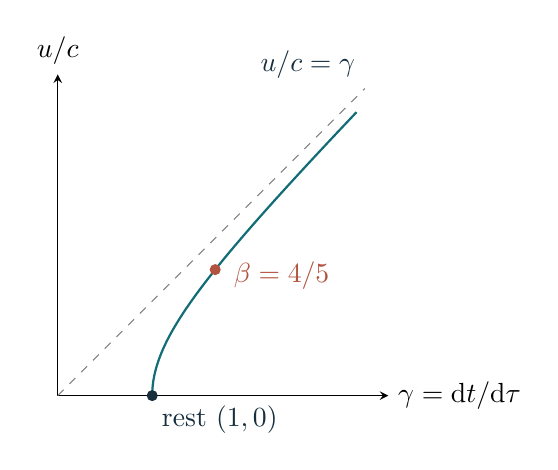
\begin{tikzpicture}[x=1.2cm,y=1.2cm,>=stealth]
    \draw[->] (0,0)--(3.5,0) node[right] {$\gamma=\mathrm{d}t/\mathrm{d}\tau$};
    \draw[->] (0,0)--(0,3.4) node[above] {$u/c$};
    \draw[dashed,gray] (0,0)--(3.25,3.25) node[above left,text=ink] {$u/c=\gamma$};
    \draw[thick,teal,domain=0:0.95,samples=100,smooth]
      plot ({1/sqrt(1-\x*\x)},{\x/sqrt(1-\x*\x)});
    \fill[ink] (1,0) circle (2pt) node[below right] {rest $(1,0)$};
    \fill[rust] (1.6667,1.3333) circle (2pt);
    \node[anchor=west,rust] at (1.76,1.27) {$\beta=4/5$};
  \end{tikzpicture}
  \caption{The curve is the nonnegative-momentum portion of the future massive-particle mass shell, $\gamma^2-(u/c)^2=1$. The dashed null line $u/c=\gamma$ is an asymptote, not a finite massive-particle state. The marked $\beta=4/5$ point is $(5/3,4/3)$. Axes use equal units.}
  \label{fig:mass-shell-hyperbola}
\end{figure}

Equal changes in $\eta$ parameterize equal rapidity steps, not equal Euclidean arc lengths in Fig.~\ref{fig:mass-shell-hyperbola}. The line $u/c=\gamma$ corresponds formally to $\beta=1$ and is approached only as $\eta\to\infty$. Along a null worldline, $\mathrm{d}\tau=0$, so proper time cannot parametrize the trajectory and $\mathrm{d}x/\mathrm{d}\tau$ is undefined. A photon is therefore not a finite point on this massive-particle curve.

\section{The reciprocal squeeze factor}
\label{sec:squeeze}

For positive rapidity, define the dimensionless squeeze factor
\begin{equation}
  k\equiv e^\eta>1.
  \label{eq:k-definition}
\end{equation}
The name indicates the exponential parameter associated with a boost; $k$ is not a wave number. The hyperbolic functions in Eqs.~\eqref{eq:gamma-cosh}--\eqref{eq:u-sinh} become
\begin{equation}
  \gamma=\frac{k+k^{-1}}{2},
  \qquad
  \frac{u}{c}=\frac{k-k^{-1}}{2},
  \qquad
  \beta=\frac{u/c}{\gamma}=\frac{k^2-1}{k^2+1}.
  \label{eq:k-kinematics}
\end{equation}
For example, $k=3$ gives $\beta=(9-1)/(9+1)=4/5$, $\gamma=5/3$, and $u/c=4/3$.

The energy--momentum form makes the reciprocal structure especially direct. From Eqs.~\eqref{eq:energy-momentum-definitions}, \eqref{eq:gamma-cosh}, and \eqref{eq:u-sinh},
\begin{align}
  \frac{E+pc}{mc^2}
  &=\gamma+\frac{u}{c}
   =\cosh\eta+\sinh\eta=e^\eta=k,
  \label{eq:light-cone-plus}\\
  \frac{E-pc}{mc^2}
  &=\gamma-\frac{u}{c}
   =\cosh\eta-\sinh\eta=e^{-\eta}=k^{-1}.
  \label{eq:light-cone-minus}
\end{align}
Multiplying these equations recovers the invariant:
\begin{equation}
  \frac{(E+pc)(E-pc)}{m^2c^4}=k\,k^{-1}=1,
  \qquad E^2-p^2c^2=m^2c^4.
  \label{eq:reciprocal-invariant}
\end{equation}
The two light-cone combinations are positive for a future-directed massive particle. Their product fixes the invariant mass; their ratio records the rapidity:
\begin{equation}
  e^{2\eta}=\frac{E+pc}{E-pc}.
  \label{eq:rapidity-energy-ratio}
\end{equation}

\section{Collinear boost composition}
\label{sec:composition}

Let an active boost of positive rapidity $\xi$ act on a momentum state while the laboratory coordinates remain fixed. With primes denoting the transformed state, the energy--momentum column transforms as
\begin{equation}
  \begin{pmatrix} E'/c \\ p' \end{pmatrix}
  =\begin{pmatrix}
    \cosh\xi & \sinh\xi \\ \sinh\xi & \cosh\xi
  \end{pmatrix}
  \begin{pmatrix} E/c \\ p \end{pmatrix},
  \qquad
  E'\pm p'c=e^{\pm\xi}(E\pm pc).
  \label{eq:active-boost}
\end{equation}
Thus the two light-cone components are scaled reciprocally. The boost matrices obey $\mathcal{B}(\xi_2)\mathcal{B}(\xi_1)=\mathcal{B}(\xi_1+\xi_2)$; a passive coordinate transformation into a frame moving at positive rapidity uses $\mathcal{B}(-\xi)$ instead.

Let two active same-direction boosts have rapidities $\eta_1$ and $\eta_2$, corresponding to $\beta_i=\tanh\eta_i$. Applying the hyperbolic tangent addition identity gives
\begin{align}
  \tanh(\eta_1+\eta_2)
  &=\frac{\tanh\eta_1+\tanh\eta_2}
          {1+\tanh\eta_1\tanh\eta_2} \\
  &=\frac{\beta_1+\beta_2}{1+\beta_1\beta_2}.
  \label{eq:rapidity-composition}
\end{align}
This is the one-dimensional Einstein velocity-addition law. Therefore the total rapidity is $\eta_1+\eta_2$. This additivity is restricted to collinear boosts; general non-collinear boosts do not reduce to this scalar rule.

If each active boost has the same positive rapidity $\eta=\ln k$ and the particle starts at rest, after $n$ steps,
\begin{equation}
  \eta_n=n\eta=n\ln k,
  \qquad
  K_n\equiv e^{\eta_n}=k^n.
  \label{eq:accumulated-squeeze}
\end{equation}
Substituting $K_n$ for $k$ in Eq.~\eqref{eq:k-kinematics} gives the complete ladder:
\begin{equation}
  \beta_n=\frac{K_n^2-1}{K_n^2+1},
  \qquad
  \gamma_n=\frac{K_n^2+1}{2K_n},
  \qquad
  \frac{u_n}{c}=\frac{K_n^2-1}{2K_n}.
  \label{eq:ladder-general}
\end{equation}
The equivalent forms in terms of the per-step factor are
\begin{equation}
  \beta_n=\frac{k^{2n}-1}{k^{2n}+1},
  \qquad
  \gamma_n=\frac{k^{2n}+1}{2k^n},
  \qquad
  \frac{u_n}{c}=\frac{k^{2n}-1}{2k^n}.
  \label{eq:ladder-k-n}
\end{equation}
At $n=0$, $K_n=1$, so $(\beta_0,\gamma_0,u_0)=(0,1,0)$, the rest state. Every finite rung with $k>1$ has $0\leq\beta_n<1$.

Exact kinematic values and energy ratios for both ladders appear in Table~\ref{tab:exact-ladders}.

The table shows how the additive parameter and nonlinear velocity sequence differ. For instance, two boosts with $k=3$ produce $\beta_2=40/41$, not twice the first-rung velocity $2(4/5)$. Rapidity, rather than ordinary velocity, is the quantity being repeated in equal increments.

\section{The energy--momentum triangle}
\label{sec:triangle}

At rung $n$, the energy and momentum are
\begin{equation}
  \frac{E_n}{mc^2}=\gamma_n=\frac{K_n^2+1}{2K_n},
  \qquad
  \frac{p_nc}{mc^2}=\frac{u_n}{c}=\frac{K_n^2-1}{2K_n}.
  \label{eq:rung-energy-momentum}
\end{equation}
Thus the ratio of rest energy to momentum times $c$ to total energy is
\begin{equation}
  mc^2: p_nc : E_n
  =1:\frac{K_n^2-1}{2K_n}:\frac{K_n^2+1}{2K_n}
  =2K_n:(K_n^2-1):(K_n^2+1).
  \label{eq:triangle-ratio}
\end{equation}
The last form is obtained by multiplying every term by the same positive factor $2K_n$. It expresses a ratio and does not change $m$ or any physical energy.

The corresponding sides satisfy the exact identity
\begin{equation}
  \begin{aligned}
    (2K_n)^2+(K_n^2-1)^2
    &=4K_n^2+(K_n^4-2K_n^2+1) \\
    &=K_n^4+2K_n^2+1=(K_n^2+1)^2.
  \end{aligned}
  \label{eq:pythagorean-identity}
\end{equation}
For $n\geq1$, this is a Euclidean right-triangle relation among three positive energy magnitudes: $mc^2$ and $p_nc$ are the perpendicular legs, and $E_n$ is the hypotenuse. At $n=0$ the momentum leg vanishes. The diagram is not a trajectory in physical space or a Minkowski spacetime diagram; it displays the invariant after moving the momentum term to the other side.

\begin{figure}[ht]
  \centering
  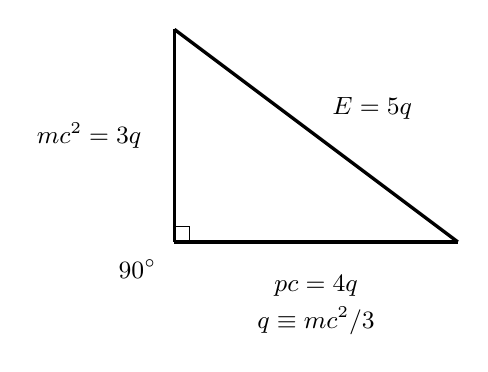
\begin{tikzpicture}[scale=0.9,every node/.style={font=\small}]
    \coordinate (O) at (0,0);
    \coordinate (A) at (0,3);
    \coordinate (B) at (4,0);
    \draw[very thick] (O)--(A) node[midway,left=8pt] {$mc^2=3q$};
    \draw[very thick] (O)--(B) node[midway,below=8pt] {$pc=4q$};
    \draw[very thick] (A)--(B) node[midway,above right=2pt] {$E=5q$};
    \draw (0,0.22)--(0.22,0.22)--(0.22,0);
    \node[below left=3pt] at (O) {$90^\circ$};
    \node[below=20pt] at (2,0) {$q\equiv mc^2/3$};
  \end{tikzpicture}
  \caption{The first $k=3$ rung drawn as a $3{:}4{:}5$ energy triangle. The scale $q$ is a common unit for the displayed ratio.}
  \label{fig:345-triangle}
\end{figure}

For integer $K_n>1$, the sides form a nondegenerate integer Pythagorean triple before reduction. At the rest rung $n=0$, $K_0=1$ gives the degenerate ratio $2:0:2$, or $1:0:1$ after reduction. The table lists the exact kinematic values and reduced energy ratios in the fixed order rest energy : $pc$ : total energy.

\begin{table}[ht]
  \centering
  \scriptsize
  \setlength{\tabcolsep}{2.5pt}
  \begin{minipage}[t]{0.49\linewidth}
    \centering
    \begin{tabular}{@{}cccccc@{}}
      \toprule
      \multicolumn{6}{c}{$k=2$ ladder} \\
      \midrule
      $n$ & $K_n$ & $\beta_n$ & $\gamma_n$ & $u_n/c$ & ratio \\
      \midrule
      1 & 2 & $3/5$ & $5/4$ & $3/4$ & $4:3:5$ \\
      2 & 4 & $15/17$ & $17/8$ & $15/8$ & $8:15:17$ \\
      3 & 8 & $63/65$ & $65/16$ & $63/16$ & $16:63:65$ \\
      \bottomrule
    \end{tabular}
  \end{minipage}\hfill
  \begin{minipage}[t]{0.49\linewidth}
    \centering
    \begin{tabular}{@{}cccccc@{}}
      \toprule
      \multicolumn{6}{c}{$k=3$ ladder} \\
      \midrule
      $n$ & $K_n$ & $\beta_n$ & $\gamma_n$ & $u_n/c$ & ratio \\
      \midrule
      1 & 3 & $4/5$ & $5/3$ & $4/3$ & $3:4:5$ \\
      2 & 9 & $40/41$ & $41/9$ & $40/9$ & $9:40:41$ \\
      3 & 27 & $364/365$ & $365/27$ & $364/27$ & $27:364:365$ \\
      \bottomrule
    \end{tabular}
  \end{minipage}
  \caption{Exact ladder values and reduced energy ratios. Each ratio is ordered $mc^2:pc:E$ for the displayed rungs.}
  \label{tab:exact-ladders}
\end{table}

The ladders can also be connected by unequal steps: rapidities $\ln(3/2)$ and $\ln2$ add to $\ln3$, so their combined state is the first rung of the $k=3$ ladder. Appendix~\ref{app:extensions} works through the intermediate $12:5:13$ ratio and the velocity addition explicitly.

For $k=3$ and $n=1$, Eq.~\eqref{eq:ladder-general} gives $\beta=4/5$, $\gamma=5/3$, and $u/c=4/3$. The energy ratio before common-factor reduction is $6:8:10$, which reduces to $3:4:5$. The broader ladder shows that this familiar ratio is one member of a sequence, rather than an isolated identity.

\section{The bridge to proper velocity}
\label{sec:proper-velocity-bridge}

Proper velocity is already present in the hyperbolic parametrization:
\begin{equation}
  u=c\sinh\eta,
  \qquad
  \gamma=\frac{\mathrm{d}t}{\mathrm{d}\tau}=\cosh\eta,
  \qquad
  v=c\tanh\eta.
  \label{eq:proper-velocity-rapidity}
\end{equation}
Eliminating $\eta$ gives
\begin{equation}
  v=\frac{u}{\sqrt{1+(u/c)^2}},
  \qquad
  \frac{u}{c}=\gamma\beta.
  \label{eq:v-from-u}
\end{equation}
These identities distinguish ordinary velocity from proper velocity. A finite $u$ can have magnitude greater than $c$ without implying a superluminal laboratory velocity; Eq.~\eqref{eq:v-from-u} gives $|v|<c$ for every finite $u$. At the $k=3$, $n=1$ rung, $u=4c/3$ while $v=4c/5$.

The role of this section is to establish the mathematical bridge: rapidity simultaneously parameterizes ordinary velocity, the clock ratio $\mathrm{d}t/\mathrm{d}\tau$, and celerity. The present treatment does not derive a force law or a travel-time model.

\section{Approach to the light-speed boundary}
\label{sec:light-limit}

From Eq.~\eqref{eq:ladder-general}, the gap between the speed ratio and unity is exactly
\begin{equation}
  1-\beta_n=\frac{2}{K_n^2+1}=\frac{2}{k^{2n}+1}>0
  \qquad\text{for every finite }n.
  \label{eq:finite-rung-gap}
\end{equation}
For fixed $k>1$, $K_n=k^n\to\infty$ as $n\to\infty$, so
\begin{equation}
  \beta_n\longrightarrow1^{-},
  \qquad
  \gamma_n=\frac{K_n+K_n^{-1}}{2}\longrightarrow\infty,
  \qquad
  \frac{u_n}{c}=\frac{K_n-K_n^{-1}}{2}\longrightarrow\infty.
  \label{eq:asymptotic-limit}
\end{equation}
The light-speed boundary is therefore a limit of the massive-particle sequence, not a finite rung. No finite number of equal boosts takes a massive particle to $c$.

\section{Interpretive limits and connection to later work}
\label{sec:limits}

The derivations establish a compact set of standard identities. Their interpretation should remain tied to their assumptions:
\begin{itemize}[leftmargin=*]
  \item The scalar rapidity-addition rule applies to collinear boosts. Non-collinear boost composition has additional structure and is outside this treatment.
  \item The squeeze factor $k=e^\eta$ is a reparameterization of a boost, not an independently measured substance or a wave number.
  \item The integer triangles are ratios of energy magnitudes. Reducing a triple does not rescale the particle's invariant mass or change the physical state.
  \item Proper velocity can exceed $c$ because it divides laboratory displacement by particle proper time. The measured laboratory velocity remains subluminal for a massive particle.
  \item Repeated boosts specify kinematic states. In a chosen laboratory frame, their endpoint energies determine the particle's net energy change: from rest, $E_n-E_0=mc^2(\gamma_n-1)$, and between rungs $E_{n+1}-E_n=mc^2[\cosh((n+1)\eta)-\cosh(n\eta)]$. They do not specify the force history, duration, acceleration mechanism, losses, or total apparatus energy cost. A passive change of frame alone does not transfer energy to the particle.
  \item The null asymptote is not a massive-particle state; photons have neither a proper-time parameter nor a celerity defined by $\mathrm{d}x/\mathrm{d}\tau$.
\end{itemize}

The proper-velocity relation is the natural next step after the ladder. The same rapidity that makes boost composition additive also makes $u/c=\sinh\eta$ and $\mathrm{d}t/\mathrm{d}\tau=\cosh\eta$ immediate. This continuity of notation is why the ladder can serve as a conceptual and algebraic foundation for the later Proper Velocity material, while leaving that work's additional physical examples to its own treatment.

\section{Conclusion}

The mass-shell invariant for a massive particle in one-dimensional flat-spacetime motion is a hyperbola. Rapidity parametrizes that hyperbola through $\beta=\tanh\eta$, $\gamma=\cosh\eta$, and $u/c=\sinh\eta$. Exponentiating rapidity gives reciprocal light-cone factors $k$ and $k^{-1}$, while same-direction boost composition adds rapidities and multiplies their factors. After $n$ identical steps, $K_n=k^n$ determines the speed, clock ratio, and proper velocity exactly.

The same formulas rewrite the energy--momentum invariant as a right-triangle relation. Integer accumulated squeeze factors produce integer Pythagorean ratios, with the $3{:}4{:}5$ electron example appearing as the first rung for $k=3$. All finite rungs remain subluminal; the light-speed limit requires infinitely many steps. Proper velocity provides a direct bridge from this ladder to later work, but neither the ladder nor the triangle is a new dynamical law. Their value is as a transparent organization of familiar relativistic structure.

\appendix

\section{A mixed-boost bridge and the Euclidean triangle angle}
\label{app:extensions}

The two illustrative ladders can be joined with unequal positive rapidity steps. Let the first boost have squeeze factor $k_1=3/2$ and the second $k_2=2$. Their total rapidity and accumulated factor are
\begin{equation}
  \eta_{\mathrm{tot}}=\ln(3/2)+\ln2=\ln3,
  \qquad
  K_{\mathrm{tot}}=k_1k_2=3.
  \label{eq:mixed-boost-total}
\end{equation}
The intermediate $k_1=3/2$ state has
\begin{equation}
  \beta_1=\frac{(3/2)^2-1}{(3/2)^2+1}=\frac{5}{13},
  \qquad
  \gamma_1=\frac{13}{12},
  \qquad
  \frac{u_1}{c}=\frac{5}{12},
  \qquad
  mc^2:p_1c:E_1=12:5:13.
  \label{eq:mixed-boost-intermediate}
\end{equation}
The ratio is written in the manuscript's fixed order, rest energy : momentum times $c$ : total energy. It is the integer triple conventionally named $5$--$12$--$13$, with the two legs reversed in this label order.

The next boost has $k_2=2$ and hence $\beta_2=3/5$. Applying velocity addition to the intermediate state gives
\begin{align}
  \beta_{\mathrm{tot}}
  &=\frac{\beta_1+\beta_2}{1+\beta_1\beta_2}
   =\frac{5/13+3/5}{1+(5/13)(3/5)} \\
  &=\frac{64/65}{80/65}=\frac45.
  \label{eq:mixed-boost-velocity}
\end{align}
The final rapidity is $\ln3$, exactly the first rung of the $k=3$ ladder, and the endpoint ratio is $3:4:5$. This example shows that a fixed integer per-step factor is a convenient ladder choice, not a requirement for composing boosts or obtaining integer energy ratios.

For the Euclidean energy triangle, let $\theta$ be the angle opposite the momentum leg $pc$. From the side definitions and rapidity identities,
\begin{equation}
  \tan\theta=\frac{pc}{mc^2}=\sinh\eta,
  \qquad
  \sin\theta=\frac{pc}{E}=\beta=\tanh\eta.
  \label{eq:triangle-angle-rapidity}
\end{equation}
Thus $\theta$ and $\eta$ are distinct angles: at the $k=3$ rung, $\eta=\ln3$ whereas $\theta=\arctan(4/3)\simeq53.13^\circ$. The Euclidean triangle represents the energy invariant, while rapidity is the hyperbolic parameter that adds under collinear boosts.

\section{Repeated velocity addition}
\label{app:boost-composition}

For a fixed positive step $\eta=\ln k$, start at rest with $\eta_0=0$ and $K_0=1$. If after $n$ active boosts $\eta_n=n\eta$, one more boost gives
\begin{equation}
  \eta_{n+1}=\eta_n+\eta=(n+1)\eta,
  \qquad
  K_{n+1}=K_n k=k^{n+1}.
  \label{eq:appendix-induction}
\end{equation}
By induction, $\eta_n=n\eta$ and $K_n=k^n$ for every nonnegative integer $n$. Substitution into the one-rung formulas gives Eq.~\eqref{eq:ladder-general}.

\begin{thebibliography}{9}
\small
\setstretch{1.0}
\raggedright
\urlstyle{same}

\bibitem{Tong}
D. Tong,
\emph{Dynamics and Relativity},
Chapter 7, §§7.3.2 and 7.4.5, lecture notes, University of Cambridge,
available at \href{https://davidtong.org/teaching/dynamics-and-relativity/}{davidtong.org/teaching/dynamics-and-relativity/}.

\bibitem{Dray}
T. Dray,
\emph{The Geometry of Special Relativity},
section ``Velocity Addition,'' Oregon State University,
available at \href{https://sites.science.oregonstate.edu/physics/coursewikis/GSR/book/content/vaddition.html}{sites.science.oregonstate.edu/physics/coursewikis/GSR/book/content/vaddition.html}.

\end{thebibliography}

\end{document}